\documentclass[10pt,a4paper]{article}
\usepackage[utf8]{inputenc}
\usepackage[french]{babel}
\usepackage[left=2cm,right=2cm,top=2cm,bottom=2cm]{geometry}
\usepackage{hyperref}
\usepackage{graphicx}
\usepackage{listings}

% \usepackage{fancyhdr}
% \fancyhead{}
% \fancyfoot{}
% \fancyhead[L]{
\includegraphics[scale=0.03]{../image/logo_iutbeziers.png}}
% \fancyhead[C]{Rapport de Stage - SuperBeeLive}
% 
% \fancyfoot[L]{\small Olivia SERENELLI-PESIN \normalsize}
% \fancyfoot[R]{\thepage/\pageref{LastPage}}
% %\fancyfoot[C]{\includegraphics[scale=0.03]{../images/logo/logo_abeille.png}}
% \renewcommand{\footrulewidth}{0pt}
% \renewcommand{\headrulewidth}{0,4pt}
% 
% %Indique qu'il faut appliquer le style sur tout le doc 
% \makeatletter
% \let\ps@plain=\ps@fancy
% \makeatother

%opening
    \title{MONITOR YOUR INFRA}
\author{Nicolas Vadkerti Quentin Risdorfer}
\usepackage{listings} % Required for inserting code snippets
\usepackage[usenames,dvipsnames]{color} % Required for specifying custom colors and referring to colors by name

\definecolor{DarkGreen}{rgb}{0.0,0.4,0.0} % Comment color
\definecolor{highlight}{RGB}{255,251,204} % Code highlight color

\lstdefinestyle{Style1}{ % Define a style for your code snippet, multiple definitions can be made if, for example, you wish to insert multiple code snippets using different programming languages into one document
language=Bash, % Detects keywords, comments, strings, functions, etc for the language specified
backgroundcolor=\color{highlight}, % Set the background color for the snippet - useful for highlighting
basicstyle=\footnotesize\ttfamily, % The default font size and style of the code
breakatwhitespace=false, % If true, only allows line breaks at white space
breaklines=true, % Automatic line breaking (prevents code from protruding outside the box)
captionpos=b, % Sets the caption position: b for bottom; t for top
commentstyle=\usefont{T1}{pcr}{m}{sl}\color{DarkGreen}, % Style of comments within the code - dark green courier font
deletekeywords={}, % If you want to delete any keywords from the current language separate them by commas
%escapeinside={\%}, % This allows you to escape to LaTeX using the character in the bracket
firstnumber=1, % Line numbers begin at line 1
frame=single, % Frame around the code box, value can be: none, leftline, topline, bottomline, lines, single, shadowbox
frameround=tttt, % Rounds the corners of the frame for the top left, top right, bottom left and bottom right positions
keywordstyle=\color{Blue}\bf, % Functions are bold and blue
morekeywords={}, % Add any functions no included by default here separated by commas
numbers=left, % Location of line numbers, can take the values of: none, left, right
numbersep=10pt, % Distance of line numbers from the code box
numberstyle=\tiny\color{Gray}, % Style used for line numbers
rulecolor=\color{black}, % Frame border color
showstringspaces=false, % Don't put marks in string spaces
showtabs=false, % Display tabs in the code as lines
stepnumber=5, % The step distance between line numbers, i.e. how often will lines be numbered
stringstyle=\color{Purple}, % Strings are purple
tabsize=2
% literate={á}{{\'a}}1 {ã}{{\~a}}1 {é}{{\'e}}1,
% inputencoding=utf8
}

\newcommand{\insertcode}[2]{\begin{itemize}\item[]\lstinputlisting[caption=#2,label=#1,style=Style1]{#1}\end{itemize}} 


% \insertcode{"Scripts/example.pl"}{Nena would be proud.} 

\begin{document}

\maketitle


\url{https://github.com/SlaynPool/CR_MONITOR_YOUR_INFRA}



\section{Utilisation de SNMP comme vecteur de monitoring}
\subsection{Installez le client SNMP sous Linux}

\insertcode{commande/1.txt}{Installation d'un Client}

\insertcode{commande/2.txt}{Test d'interogation}

Pour Autoriser les connections de l'exterieur, il faut :

\insertcode{commande/3.txt}{snmpd.conf}

\section{Utilisez le client SNMP afin de visualiser les informations des machineslistées dans le "terrain de jeux"}
\subsection{Interrogation via SNMP du serveur ayant pour IP 10.6.0.1.}
\subsubsection{Dumper l’ensemble des informations du serveur distant via un snmpwalk}
\insertcode{commande/4.txt}{snmpwalk}

\subsubsection{Retrouver le système d’exploitation de la machine via un snmpget.}
\insertcode{commande/5.txt}{snmpget}

\subsubsection{Afficher l’arbre system de la mib à l’aide de la commande }
\insertcode{commande/6.txt}{Arbre de la mib SNMPv2}
\subsubsection{Traduisez en oid SNMPv2-MIB : :system et réciproquement}
\insertcode{commande/7.txt}{Traduction}

\subsubsection{Retrouvez à l’aide de snmpnetstat la liste des connections TCP et UDP du serveur distant}
\insertcode{commande/8.txt}{snmpNetstat}


\subsubsection{ quoi sert la commande snmpgetnext ? Utilisez la pour retrouvez SNMPv2-MIB : :sysContact.0}
Source : \url{man_snmpgetnext}
\begin{lstlisting}
                snmpgetnext  is  an SNMP application that uses
                    the SNMP GETNEXT request to query for informa
                    tion  on a network entity.  One or more object
                    identifiers (OIDs) may be given  as  arguments
                    on  the  command  line.  Each variable name is
                    given in the format specified in variables(5).
                    For  each  one,  the  variable that is lexico
                    graphically "next" in the remote entity's  MIB
                    will be returned.

\end{lstlisting}
La commande sert donc à afficher des informations à propos du périphérique interrogé.
\insertcode{commande/9.txt}{snmpgetnext}
\newpage


 \section{Utilisation d’OMD comme logiciel de supervision SNMP}

Paquets à installer:

mk-check-agent: \url{store.iutbeziers.fr/check-mk-agent/}

OMD: \url{http://clusterfrak.com/sysops/app_installs/omd_install/}

\subsection{Supervisez avec OMD}


Créer notre site avec OMD:
\insertcode{commande/a.txt}{Création iutbeziers}

Premiers pas:
\insertcode{commande/b.txt}{Afficher status du site}


\insertcode{commande/c.txt}{Démarrer notre site IURBEZIERS}
 
 
 
 
 

  \begin{figure}[h!]
\centering
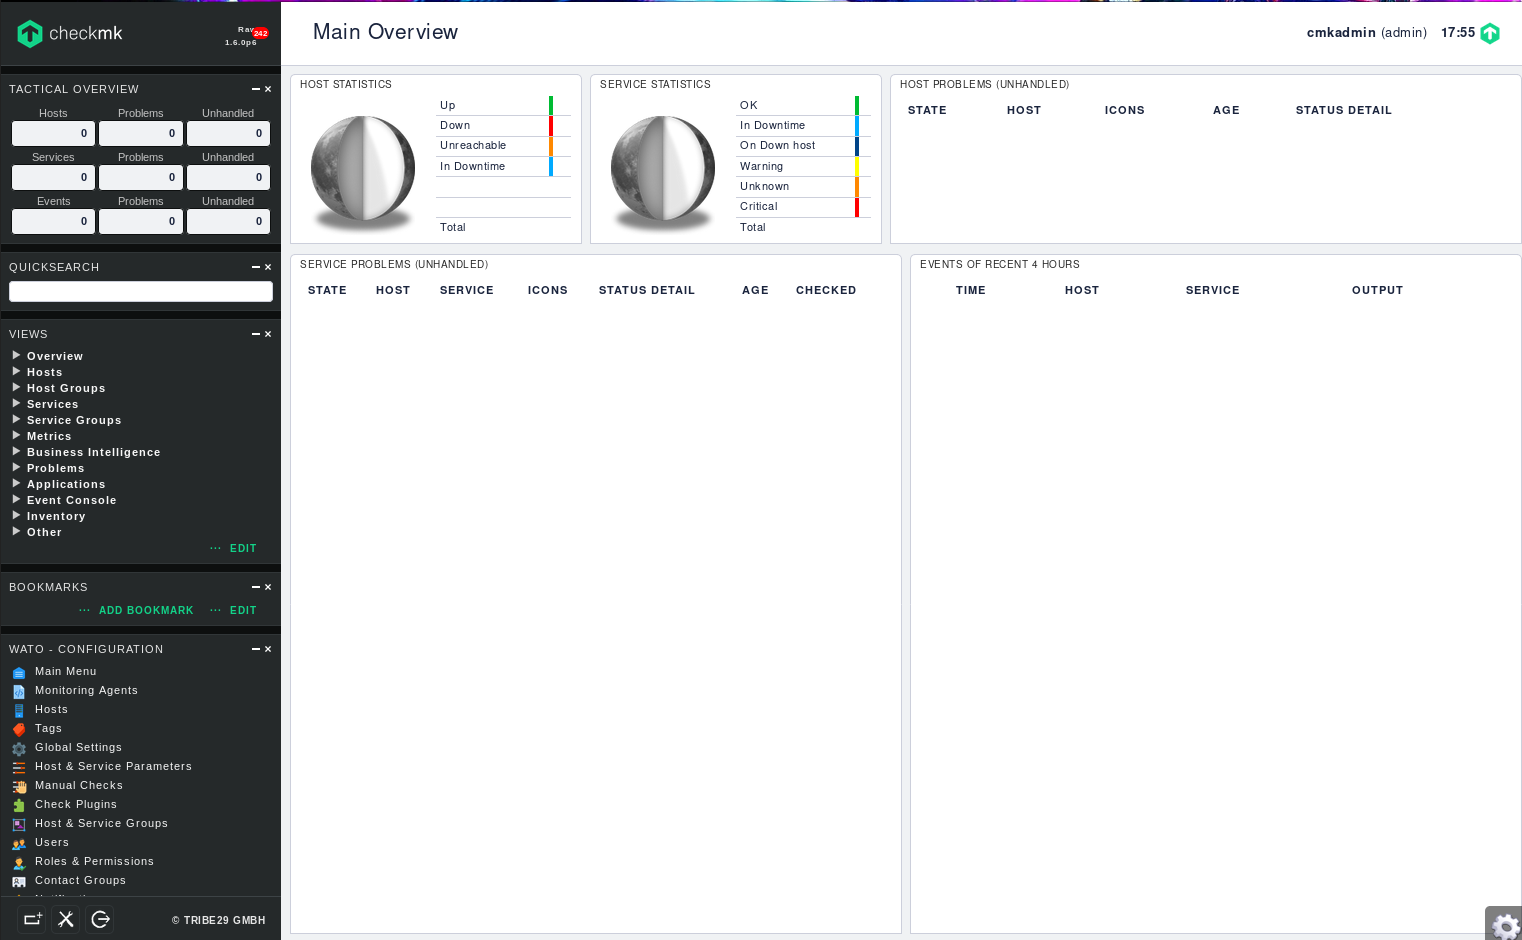
\includegraphics[scale=0.30]{screen/checkmk.png}
\caption{checkmk}
\label{fig:qos}
\end{figure}




\subsection{Quelques services Configuré}

  \begin{figure}[h!]
\centering
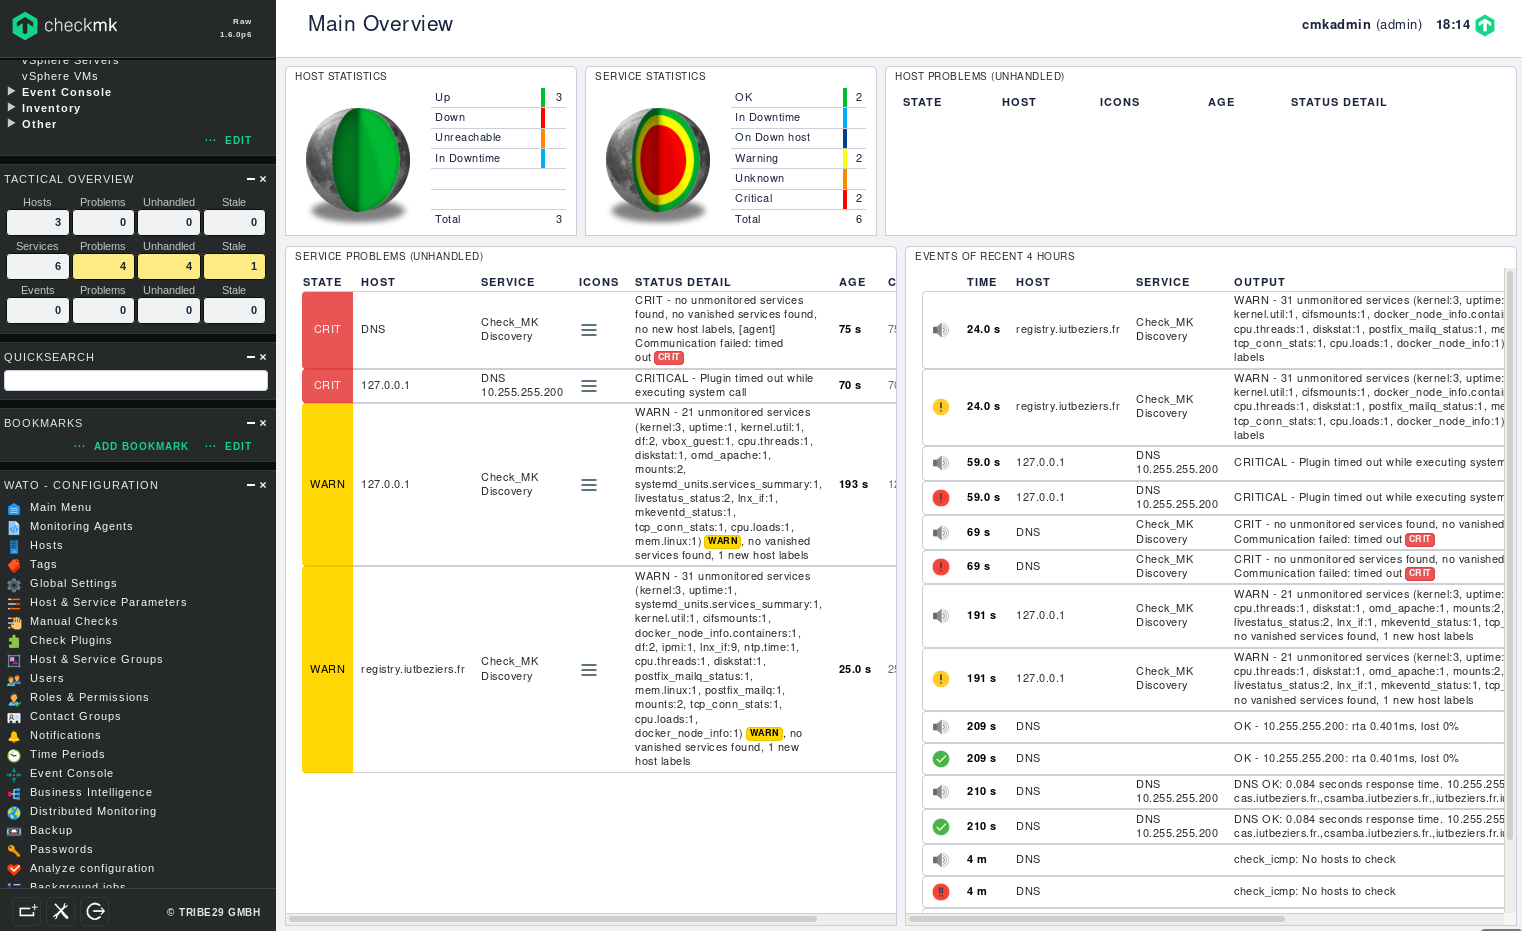
\includegraphics[scale=0.30]{screen/checkmk2.png}
\caption{checkmk}
\label{fig:qos}
\end{figure}



\newpage
\section{Métrologie de vos serveurs et postes de travail avec Grafana.}
\subsection{Installation de Grafana/influxDB côté serveur.}
\insertcode{commande/10.txt}{Installation/Utilisation de Docker}


\subsection{ Configuration de la source de données Collectd.}

En suivant le sujet de TP, 
Nous obtenons ceci 
  \begin{figure}[h!]
\centering
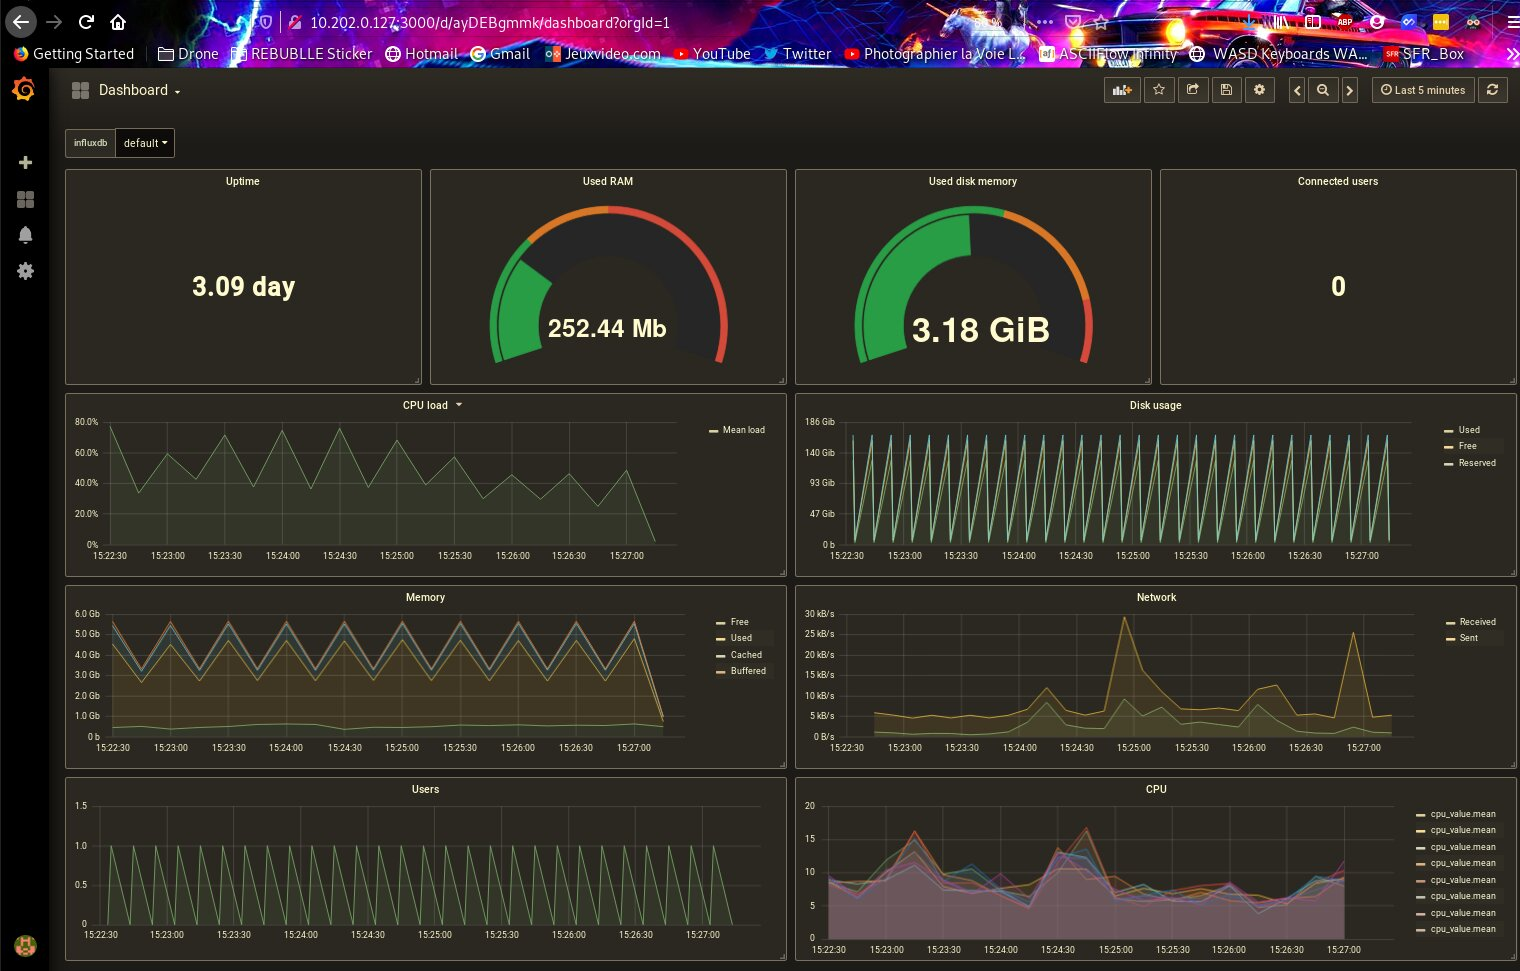
\includegraphics[scale=0.30]{screen/collectd.jpg}
\caption{Dashboard Graphana }
\label{fig:qos}
\end{figure}

\subsection{Importation d’un dashboard pour telegraf}
  \begin{figure}[h!]
\centering
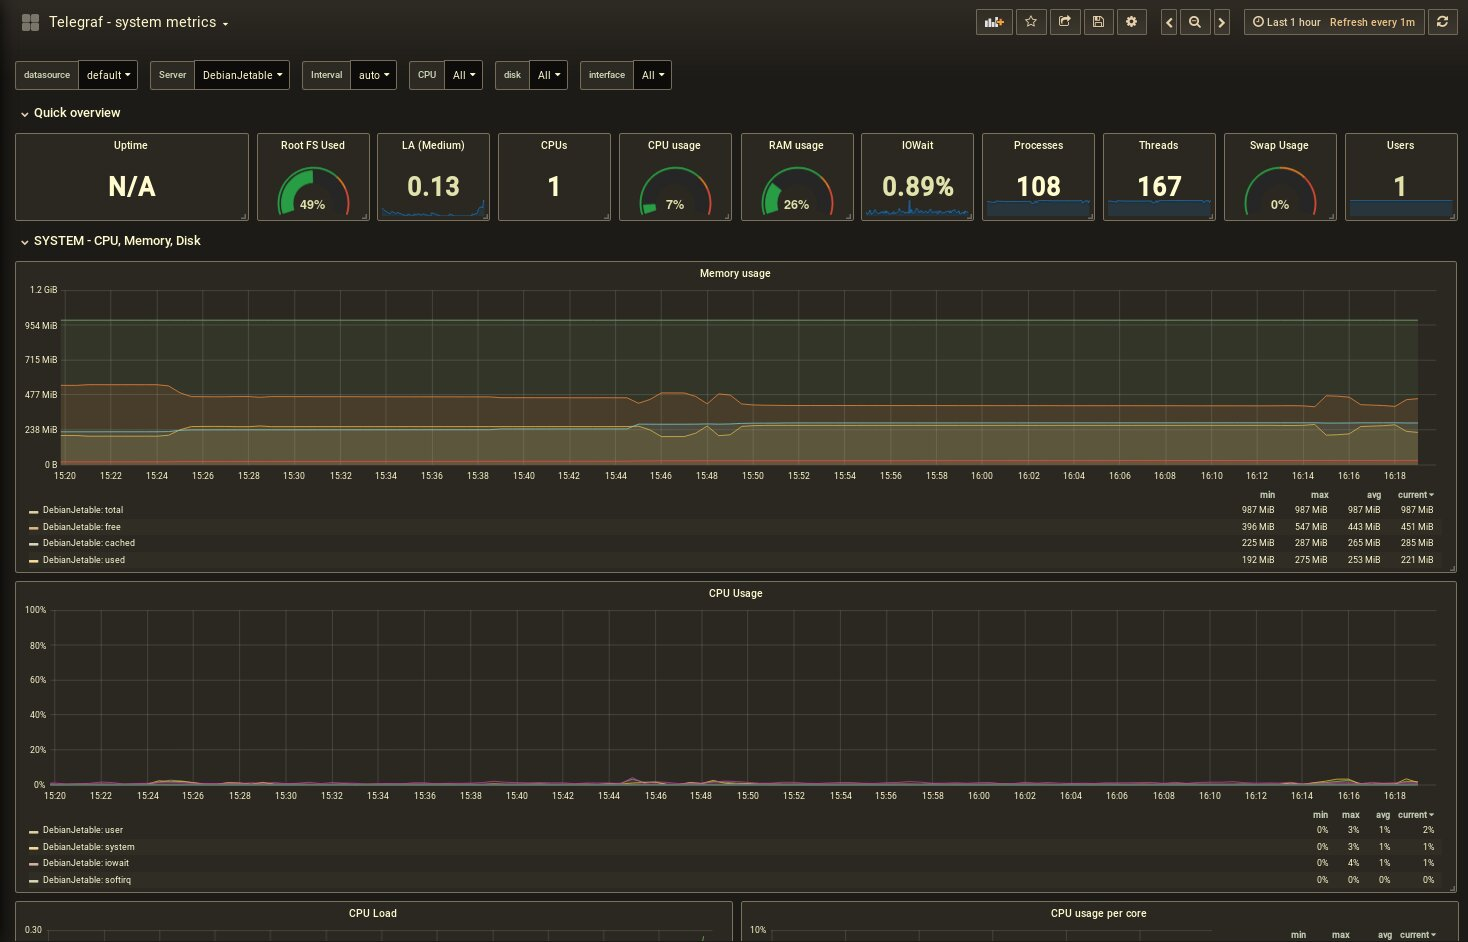
\includegraphics[scale=0.30]{screen/telegraf.jpg}
\caption{Dashboard telegraf}
\label{fig:qos}
\end{figure}





\newpage
\section{Connexion à influxDB}

\subsection{Donnez le nom des bases}
\insertcode{commande/11.txt}{Liste des Tables}

 \subsection{Lister les USERS }
 Nous n'avons pas crée d'utilisateur dans la DB mais la commande est :
 \insertcode{commande/12.txt}{Liste USERS}
 
 \subsection{Donner la liste des "time series" par base.}
 \insertcode{commande/13.txt}{SHOW SERIES}
%  \subsection{Lister Via une requete SQL les enregistrements ``bytes_recv'' groupés par tranche de 10 seconde }
%  J'ai pas trouvé de champs bytes_recv mais :
 
 \newpage
 \subsection{Enregistrements groupé par tranche de 10s }
 \insertcode{commande/14.txt}{GROUPE BY}


\end{document}


